\documentclass[14pt]{extarticle}
\usepackage{fontspec}
\usepackage[russian]{babel}
\setmainfont{Times New Roman}
\usepackage{amssymb}
\usepackage{setspace}
\usepackage{enumitem}
% \onehalfspacing
\usepackage{amsmath}
\usepackage{listings}
\usepackage{booktabs}
\usepackage{pdfpages}
\usepackage{xcolor}
\usepackage{float}
\usepackage{graphicx}
\usepackage{tikz}
\usepackage{url}
\usepackage{csquotes}
% \urlstyle{same}
\usepackage{longtable}
\usepackage{titlesec}
\usepackage{caption}
\usepackage{titletoc}
\usepackage{indentfirst}
% \usepackage[titles]{tocloft}
\usepackage[
    backend=biber,
    sorting=nty,        
    style=gost-numeric,
    % sortlocale=ru_RU,  
    language=auto,
    autolang=other
]{biblatex}
\AtBeginBibliography{\renewcommand*{\mkbibemph}[1]{#1}}
\DeclareNameAlias{default}{family-given}
\DeclareSourcemap{
  \maps[datatype=bibtex]{
    \map{
      \step[fieldsource=langid, match=ru, final]
      \step[fieldset=presort, fieldvalue={a}]
    }
    \map{
      \step[fieldsource=langid, notmatch=ru, final]
      \step[fieldset=presort, fieldvalue={b}]
    }
  }
}

\setlength{\biblabelsep}{5pt}
\addbibresource{bibl.bib}
\titleformat{\section}
  {\normalfont\fontsize{14}{17.5}\bfseries\centering}{\thesection. }{0em}{}
\titleformat{\subsection}
  {\normalfont\fontsize{14}{17.5}\bfseries}{\hspace{1.25cm}\thesubsection. }{0em}{}

% \addto\captionsrussian{\renewcommand{\contentsname}{СОДЕРЖАНИЕ}}
\setcounter{page}{2} 
\setlength{\parindent}{1.25cm}
\usepackage[right=10mm,left=30mm,top=20mm,bottom=20mm]{geometry}
\setlist[enumerate,1]{
    label=\arabic*),
      leftmargin=1.25cm,
      labelsep=0.3em,
      itemindent=0pt,
      labelwidth=0em,
      align=left,
      topsep=0pt,
      itemsep=0pt,
      parsep=0pt
}
\DeclareCaptionLabelSeparator{emdash}{ -- } 
\DeclareCaptionLabelSeparator{gostdash}{ -- }
\captionsetup[table]{
  justification=raggedright,
  singlelinecheck=false,   
  labelsep=emdash,        
  skip=0pt,              
  % font=normalsize,
  font={stretch=1.5}
}
\addto\captionsrussian{\renewcommand{\figurename}{Рисунок}}
\captionsetup[figure]{
    labelsep=gostdash,       % Рисунок 1 — Название
    justification=centering, % по центру
    singlelinecheck=false,   % не центрировать однострочные
    skip=0pt,                % без отступа
    font={stretch=1.5}
}

% \setlength{\intextsep}{0pt} % отступы вокруг плавающих объектов
\setlength{\abovecaptionskip}{0pt} % между рисунком и подписью
\setlength{\belowcaptionskip}{0pt} % после подписи
\setlength{\intextsep}{1.5pt} % отступы вокруг плавающих объектов
% \setlength{\floatsep}{0pt}
\usepackage{etoolbox}
\BeforeBeginEnvironment{figure}{\vspace{0.15cm}}
\AfterEndEnvironment{figure}{\vspace{-0.35cm}}
\titlespacing*{\section}
{0pt}{0pt}{0pt}
\titlespacing*{\subsection}
{0pt}{0pt}{0pt}
% \titlespacing*{\contentsname}{0pt}{0pt}{-2em}
\renewcommand{\baselinestretch}{1.5}
\usepackage{tocloft}
\usepackage{setspace}
\addto\captionsrussian{\renewcommand{\contentsname}{СОДЕРЖАНИЕ}}

\renewcommand{\cfttoctitlefont}{\hspace*{\fill}\fontsize{14}{21}\selectfont\bfseries}
\renewcommand{\cftaftertoctitle}{\hspace*{\fill}\null}

% Размер шрифта для элементов содержания
\renewcommand{\cftsecfont}{\fontsize{14}{21}\selectfont\bfseries}
\renewcommand{\cftsubsecfont}{\fontsize{14}{21}\selectfont}
\renewcommand{\cftsubsubsecfont}{\fontsize{14}{21}\selectfont}
\renewcommand{\cftsecpagefont}{\fontsize{14}{21}\selectfont\bfseries}
\renewcommand{\cftsubsecpagefont}{\fontsize{14}{21}\selectfont}
\renewcommand{\cftsubsubsecpagefont}{\fontsize{14}{21}\selectfont}

% Межстрочный интервал
\renewcommand{\cftbeforetoctitleskip}{0pt}
\renewcommand{\cftaftertoctitleskip}{0pt}  % Убираем отступ
\setlength{\cftbeforesecskip}{0pt}
\setlength{\cftbeforesubsecskip}{0pt}
\setlength{\cftbeforesubsubsecskip}{0pt}
\setstretch{1.5}
% \onehalfspacing
\begin{document}
\setcounter{page}{2}
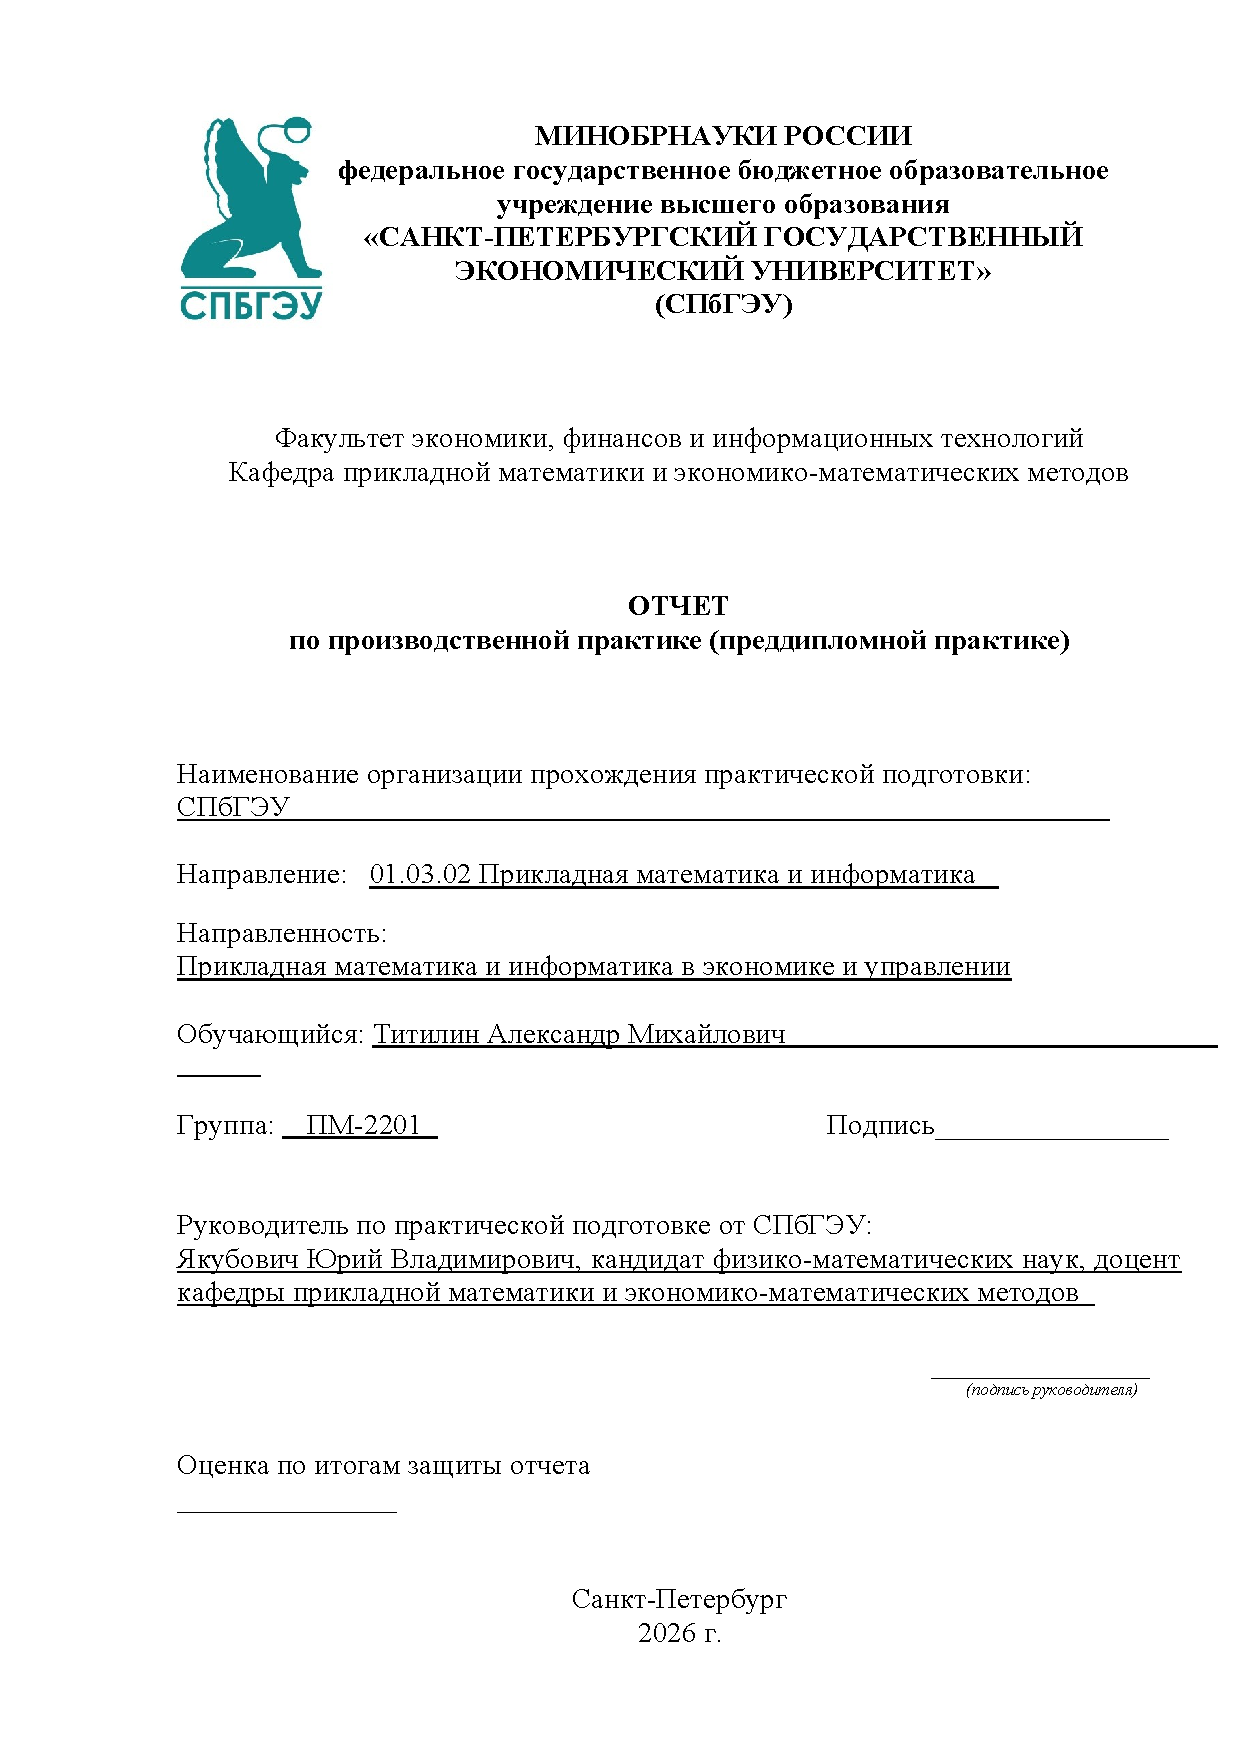
\includepdf{title1.pdf}
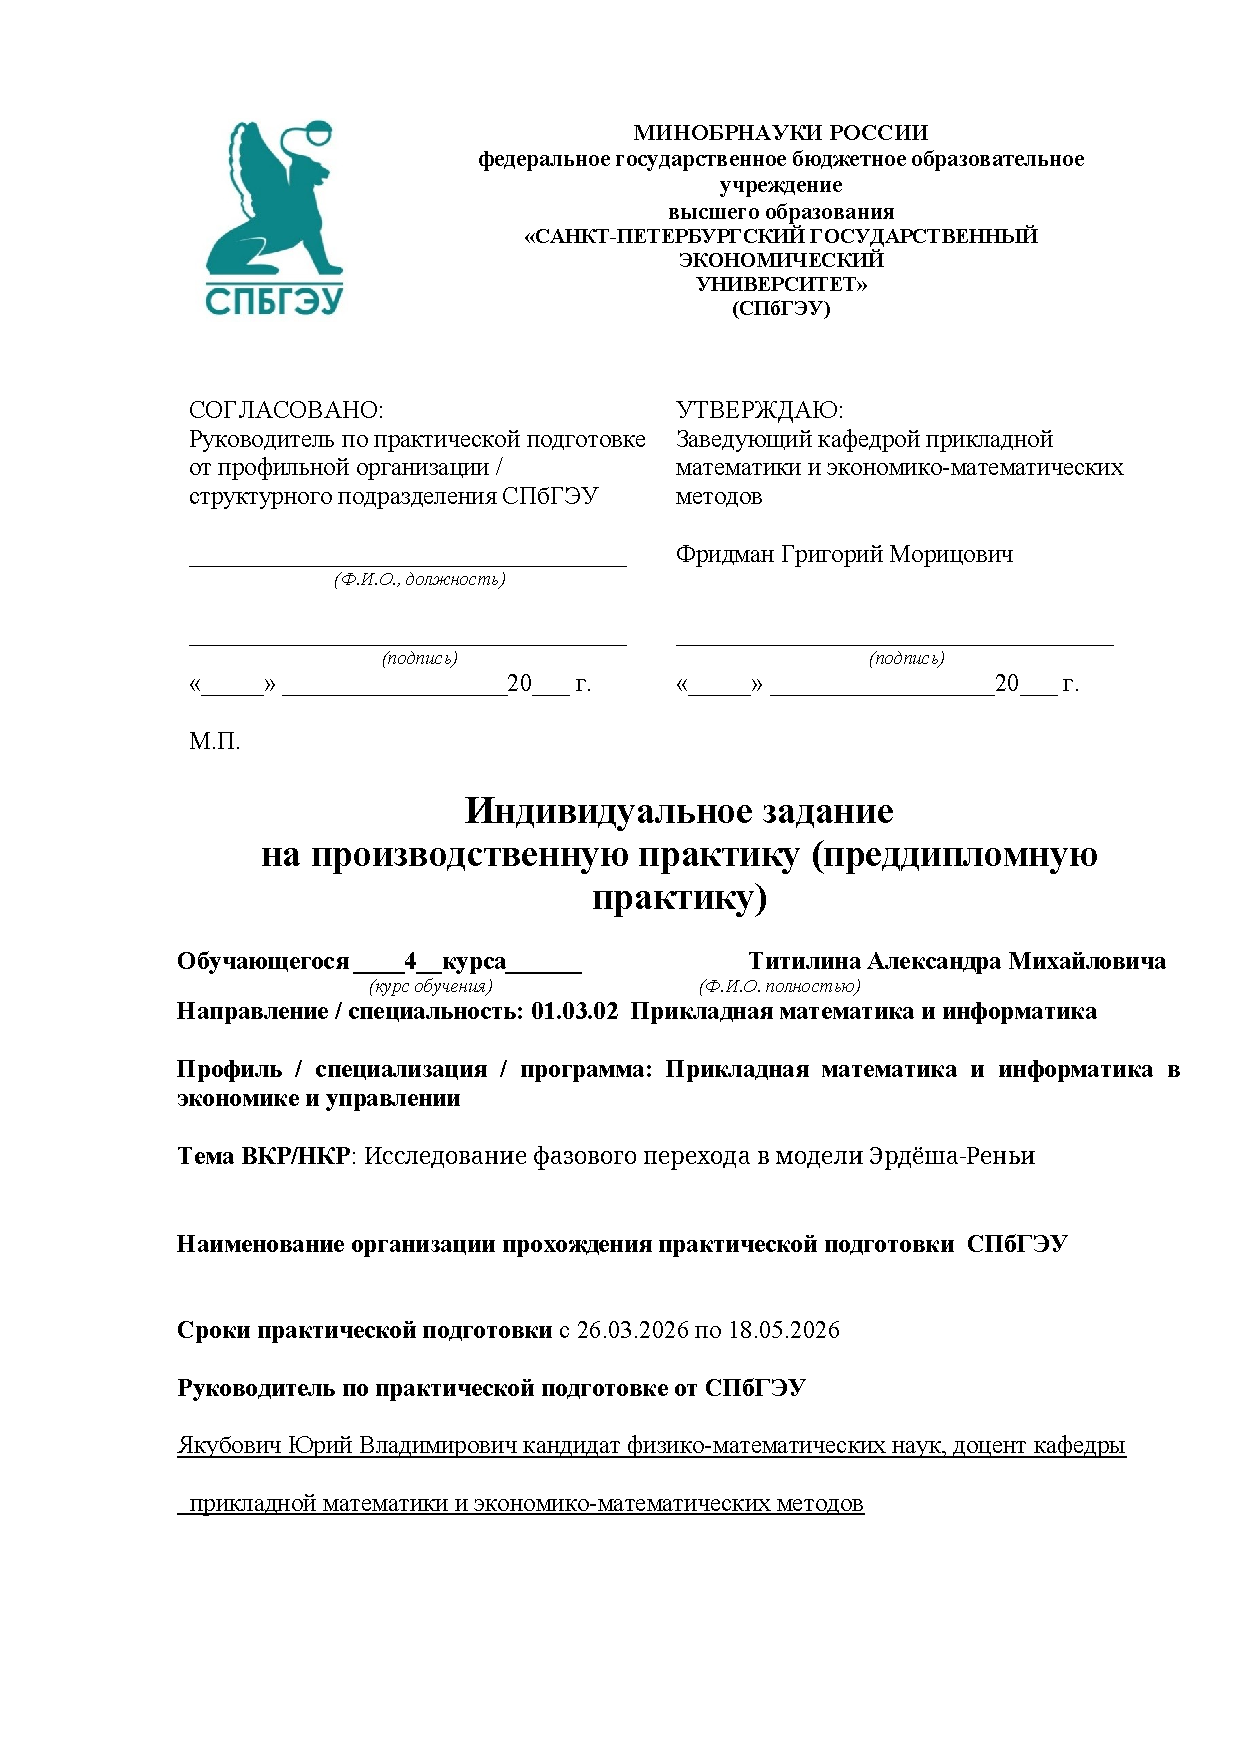
\includepdf[pages=1]{title2.pdf}
\includepdf[pages=2]{title2.pdf}
\begin{spacing}{1.5}
\tableofcontents
\end{spacing}
\pagebreak{}
\addcontentsline{toc}{section}{ВВЕДЕНИЕ}
\section*{ВВЕДЕНИЕ}
Случайные графы находят широкое приложение в различных областях,
таких как физика, биология, социальные и экономические науки. 
Наиболее теоретически исследованной моделью случайного графа является 
модель Эрдёша--Реньи $G(n,p)$, в которой строится 
неориентированный граф на $n$ вершинах, каждое ребро добавляется с
вероятностью  $p$ независимо от остальных. Данная модель имеет 
важное свойство -- фазовый переход, который заключается в резком изменении структуры графа, после достижения критического значения параметра $p$. 

Несмотря на то, что фазовый переход в модели $G(n,p)$ 
теоретически хорошо изучен, её поведение  
при конечных $n$ существенно отличается от асимптотического. Это делает численное исследование 
модели актуальным для проверки скорости сходимости теоретических
результатов.

Целью работы является численное исследование модели Эрдёша--Реньи. 
Были реализованы графы, алгоритмы на графах и вычислительный эксперимент. Также были визуализированы результаты экспериментов.
Были изучены характеристики полученных графов -- количество 
компонент связности, размер наибольшей компоненты связности, структура подграфа, построенного на вершинах из компоненты связности, размер наибольшего найденного пути, асимметричность распределения размеров наибольших компонент связности.
Для достижения цели решались следующие задачи:
\begin{enumerate}
    \item реализация генератора случайных графов 
        согласно модели $G(n,p)$ на языке программирования C++;
    \item реализация алгоритмов для вычисления характеристик графов;
    \item проведение вычислительных экспериментов;
    \item анализ и визуализация полученных данных;
\end{enumerate}

Работа состоит из введения, трёх глав, заключения и списка 
использованных источников. В первой главе рассматриваются 
основные понятия теории графов и свойства модели $G(n,p)$.
Во второй главе представлена программная реализация графов, 
вычислительного эксперимента и анализа полученных результатов.
В третьей главе приводятся результаты экспериментов.

\pagebreak
\section{МОДЕЛЬ ЭРДЁША--РЕНЬИ. ЕЁ СВОЙСТВА}
\label{g1}
В данном разделе вводятся ключевые определения и обозначения, 
излагается алгоритм поиска в глубину, используемый для нахождения 
компонент связности графа, и формулируются теоретические результаты
о свойствах модели $G(n,p)$.
\subsection{Основные определения}

Введем понятие неориентированного графа: $G=(V,E)$, где  $V = \{1, 2, \dots, n\}$ множество натуральных чисел от 
$1$ до  $n$, $E$ -- множество неориентированных ребер. Определим
путь как последовательность вершин графа, такую, что
две соседние вершины связаны ребром и каждое ребро встречается не более одного раза. Циклом называется такой путь, 
который начинается и заканчивается в одной вершине. Граф является связным, если между любыми двумя вершинами существует 
путь. Связный граф без циклов называется деревом. Подграф графа $G = (V,E)$ -- это такой граф $G' =(V',E')$,
$V' \subset V$, $E' \subset E$. Компонентой связности графа 
называется максимальный по включению связный подграф, добавление вершин в который 
нарушит связность.
\subsection{Поиск компонент связности с помощью поиска в глубину}
Рассмотрим алгоритм поиска компонент связности с помощью поиска в 
глубину. Заданы три множества $S$ -- множество посещенных вершин,
 $T$ -- множество непосещенных вершин и упорядоченное множество $U = V \setminus (S \cup T)$, организованное как стек. В начале работы алгоритма $T=V$,
 $S= U = \emptyset$. Алгоритм прекращает свою работу в случае, если
 $U \cup T = \emptyset$. Если $U$ не пусто, $v$-- последняя добавленная в  $U$ вершина, то в  $T$ 
 берется смежная вершина с $v$ вершина, удаляется из  $T$,   
 добавляется в  $U$. Если такой вершины нет, то  $v$ удаляется 
 из  $U$ и добавляется в  $S$. Если  $U$ пусто, то из 
 $T$ удаляется первая вершина и добавляется в  $U$. 
 Компонента связности находится тогда, когда множество  $U$
 становится пустым после удаления вершины.
\subsection{Свойства модели Эрдёша--Реньи}

Рассмотрим модель случайного графа  $G(n,p)$, $n$ -- количество 
вершин,  $p \in [0;1]$-- вероятность, с которой каждое ребро добавляется независимо друг от друга в граф. 
Будем говорить, что событие $\mathcal{E}_{n}$ 
происходит с высокой вероятностью, если $\lim_{n \to \infty} \text{Pr}(G \sim G(n,p) \in \mathcal{E}_{n}) =1 $. Иными
словами, вероятность события стремится к $1$ при $n \to \infty$. В статье Кривелевича и Судакова \cite{ft} были доказаны оценки размеров 
компонент связности и длины пути. Пусть $\epsilon > 0$ -- 
достаточно малое число, тогда если граф  $G$ 
создан в соответствии с моделью  $G\left(n,\frac{1-\epsilon}{n}\right)$,
то с высокой вероятностью размер всех его компонент связности не превосходит 
$\frac{7}{\epsilon^2} \ln{n}$. Если граф $G$ 
создан в соответствии с моделью  $G\left(n,\frac{1+\epsilon}{n}\right)$, то с высокой вероятностью 
этот граф содержит путь длиной хотя бы $\frac{\epsilon^2 n}{5}$ 
и имеет компоненту связности, размер которой больше чем 
$\frac{en}{2}$. Значение $p=\frac{1}{n}$ является критическим , при его достижения
структура графа меняется. При $p< \frac{1}{n}$ компоненты 
связности имеют небольшой размер, среди них много деревьев, 
после преодоления критического значения граф приобретает гигантскую компоненту связности. Также в книге Райгородского
\cite{rai} доказаны следующие свойства, если граф создан 
в соответствии с моделью $G\left(n,c\frac{\ln{n}}{n}\right)$,
то граф с высокой вероятностью связен, если $c > 1$ и несвязен, если $c < 1$. Значение $p = \frac{\ln{n}}{n}$ является фазовым переходом, после его достижение структура графа меняется. Таким 
образом в модели $G(n,p)$ существуют два 
критических значения  $p$, при которых происходит фазовый переход.
После достижения  $p = \frac{1}{n}$ появляется гигантская компонента связности, после достижения $p = \frac{\ln{n}}{n}$ 
граф становится связным.

\pagebreak{}
\section{ПРОГРАММНАЯ РЕАЛИЗАЦИЯ}
В данном разделе будет описан вычислительный эксперимент, 
реализация графов и обработка результатов экспериментов.
\subsection{Реализация графов и алгоритмов на них}

Так как для экспериментальной проверки свойств 
необходимы графы с большим количеством вершин,
готовые реализации графов, такие как
встроенные средства работы с графами в системе Wolfram Mathematica и 
библиотека языка программирования Python NetworkX,
не подходят из-за низкой производительности.
Поэтому графы были реализованы на языке программирования C++.

Графы были реализованы с использованием объектно-ориентированного подхода. Для этого был создан абстрактный класс <<BaseGraph>>, 
который имеет следующие методы:
\begin{enumerate}
    \item get\_n -- получение количества вершин;
    \item get\_n\_edges -- получение количества ребер;
    \item has\_edge -- проверка существования ребра между двумя вершинами;
    \item add\_edge -- добавление ребра между двумя вершинами;
    \item deg -- степень вершины;
    \item get\_neighbours -- получение списка вершин, смежных данной вершине;
\end{enumerate}
Данный абстрактный класс является родительским 
для класса <<Graph>>, который реализует неориентированный невзвешенный граф, представленный списками смежности. Использование
абстрактного класса позволит при необходимости 
заменить представление графа без изменения алгоритмов 
и вычислительного эксперимента.

Алгоритмы были реализованы с помощью функций, которые принимают 
на вход константную ссылку на граф и возвращают числовое значение. Были реализованреализованы следующие алгоритмы: поиск наибольшей компоненты связности, 
поиск количества компонент связности, поиск наибольшего пути 
в графе, найденном с помощью поиска в глубину, подсчет доли
деревьев среди всех компонент связности.
\subsection{Вычислительный эксперимент}

Для численного анализа модели $G(n,p)$ нужно 
много раз изучить, как изменяется граф при изменении $p$ 
в заданном диапазоне. Рассмотрим, как проводится вычислительный эксперимент:
\begin{enumerate}
        \item генерируется последовательность $U$ из 
            $ N = \frac{n(n-1)}{2}$ псевдослучайных чисел, равномерно распределенных на $[0;1]$;
        \item $p$ дискретно меняется в диапазоне  $[p_{\min}; p_{\max}]$;
        \item создается граф, в котором ребро под 
            номером $i = 1 \dots N$ существует, если
             $U_{i} < p$;
        \item для построенного графа вычисляются требуемые характеристики;
        \item результаты сохраняются в файл;
\end{enumerate}

В результате многократного повторения данного эксперимента 
получится файл, в котором каждая строка -- 
это результат эксперимента.

Такой подход к проведению вычислительного эксперимента позволит 
проследить эволюцию одного графа при изменении $p$.

Для программной реализации данного вычислительного эксперимента был создан класс <<RandomVariation>>. При инициализации получает 
на вход количество вершин графа, количество экспериментов, 
cписок границ диапазонов, название файла, в который будут записаны результаты, и функцию для вычисления требуемых характеристик графа. Для проведения эксперимента нужно использовать два метода:
<<variation>> для создания графов и вычислений характеристик и
<<save\_results>> для сохранения результатов в файл.

\subsection{Анализ и визуализация результатов экспериментов}

Для анализа и визуализации полученных данных использовался 
язык программирования Python и библиотеки 
numpy, scipy и matplotlib. Был реализован класс <<DataLoader>> 
для чтения данных из файлов. Классы для визуализации и анализа 
наследуются от него. Например, класс <<Plotter>> для визуализации 
изменения размера наибольшей компоненты связности, реализует
метод <<plot>> для создания графика с помощью библиотеки matplotlib.

\pagebreak
\section{АНАЛИЗ РЕЗУЛЬТАТОВ ЭКСПЕРИМЕНТОВ}
В разделе \ref{g1} рассмотрены теоремы, которые давали 
теоретическую оценку
характеристик графов, созданных 
в соответствии с моделью $G(n,p)$. В этом разделе будут 
показаны результаты численного исследования модели  $G(n,p)$.
\subsection{Анализ размеров наибольших компонент связности}
Рассмотрим изменение размеров наибольших компонент связности 
при $n = 10000$, $\epsilon=0.1$, $p \in [\frac{1-\epsilon}{n};\frac{1+\epsilon}{n}]$.
\begin{figure}[H] 
    \centering
    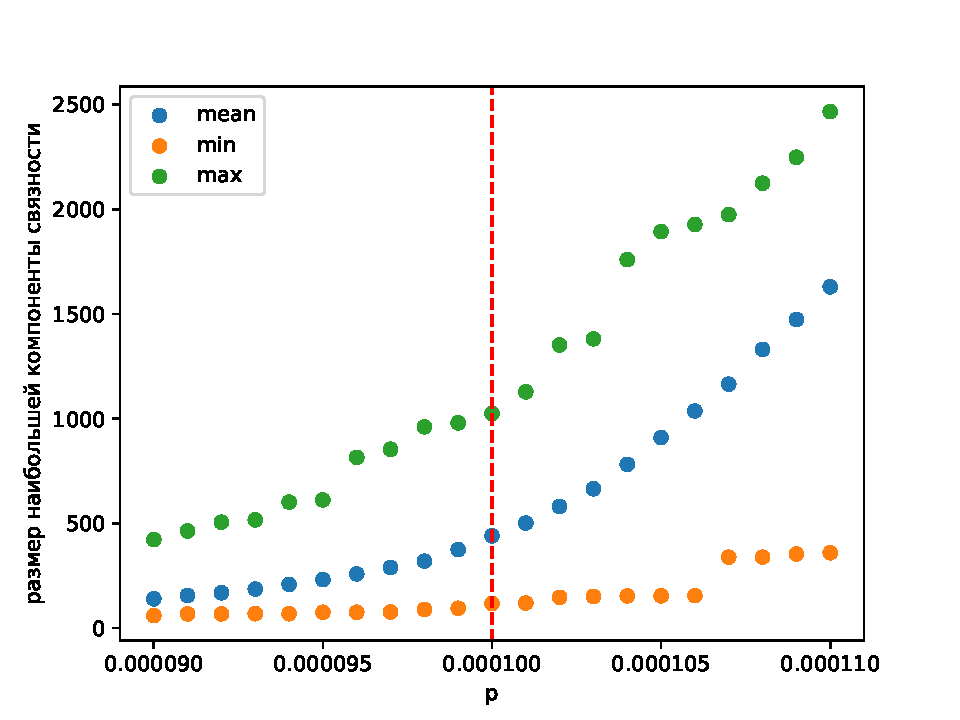
\includegraphics{../../plots/plot.pdf} 
    \caption{Изменение размера наибольшей компоненты связности}
    \label{cmp_1}
\end{figure} 
\begin{figure}[H] 
    \centering
    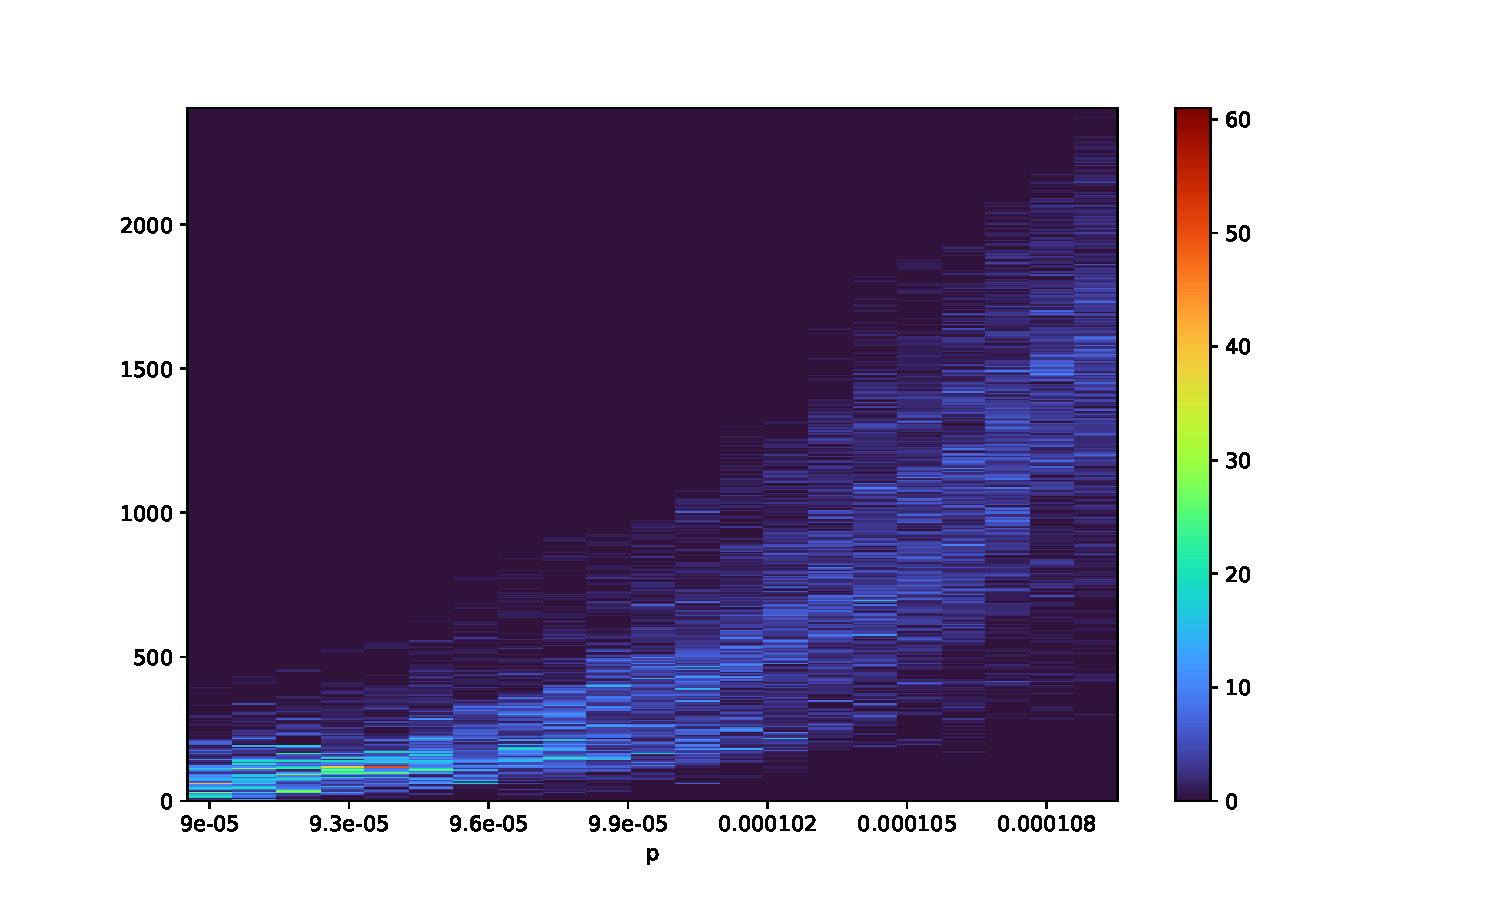
\includegraphics[scale=0.8]{../../plots/hm.pdf} 
    \caption{Тепловая карта изменения размера наибольшей компоненты связности}
    \label{hm_1}
\end{figure} 
% На рисунках \ref{cmp_1},\ref{hm_1} приведена визуализация изменений размера 
% наибольшей компоненты связности.
Из графика, изображенного на рисунке \ref{cmp_1},
можно увидеть фазовый переход в точке $p =\frac{1}{n}$, 
помеченной красной чертой. После его достижения размер наибольших компонент связности начинает расти быстрее. Тепловая 
карта, приведенная на рисунке \ref{hm_1} более подробно описывает
изменения размера наибольшей компоненты связности.

Теперь рассмотрим выполнение теорем о размерах компонент связности при $n=10000$, $\epsilon \in \{0.1,0.5,0.01\}$. Для каждого значения 
$\epsilon$ было проведено 350 экспериментов, вычислены размеры наибольших компонент связности. При $p = \frac{1-\epsilon}{n}$ 
была посчитана доля экспериментов, где размер наибольшей компоненты связности меньше теоретической оценки, при 
$p = \frac{1 + \epsilon}{n}$, доля экспериментов, где размер 
наибольшей компоненты связности больше теоретической оценки.
\begin{table}[H]
    \centering
    \caption{Результаты численного исследования размеров наибольших компонент связности}
    \begin{tabular}{|c|c|c|c|}
        \hline
        $\epsilon$ & $0.1$ & $0.5$ & $0.01$ \\
        \hline
        $p = \frac{1-\epsilon}{n}$ & $1$ &  $1$ &  $1$ \\
        \hline
        $p = \frac{1+\epsilon}{n}$ & $0.94$ & $1$ & $1$ \\
        \hline
    \end{tabular}
    \label{tab_1}
\end{table}
Как можно заметить из таблицы \ref{tab_1}, теоремы о 
размерах компонент связности выполняются почти всегда.
\subsection{Проверка симметричности распределения размера наибольших компонент связности}
\label{test}
Рассмотрим метод проверки гипотезы о симметричности выборки, описанный в статье Мяо, Гель и Гаствирта \cite{sym}.
Построим статистику $T = \frac{\overline{X} - M}{J}$, где:
\begin{enumerate}
    \item $\overline{X}$ -- выборочное среднее;
    \item $M$ -- выборочная медиана;
    \item  $J =  \sqrt{\frac{\pi}{2}} \cdot \frac{1}{n}\sum_{i=1}^{n} |X_{i} - M| $
\end{enumerate}

$H_0$ -- гипотеза о симметричности выборки, отклоняется, если
$|T| \ge \frac{z_{\frac{\alpha}{2}} \sqrt{0.5708} }{\sqrt{n} }$,
где $z_{\alpha}$ -- верхний квантиль уровня $\alpha$ стандартного нормального распределения. Для тестов, приведенных ниже, 
использовался $\alpha = 0.95$
 \begin{figure}[H] 
     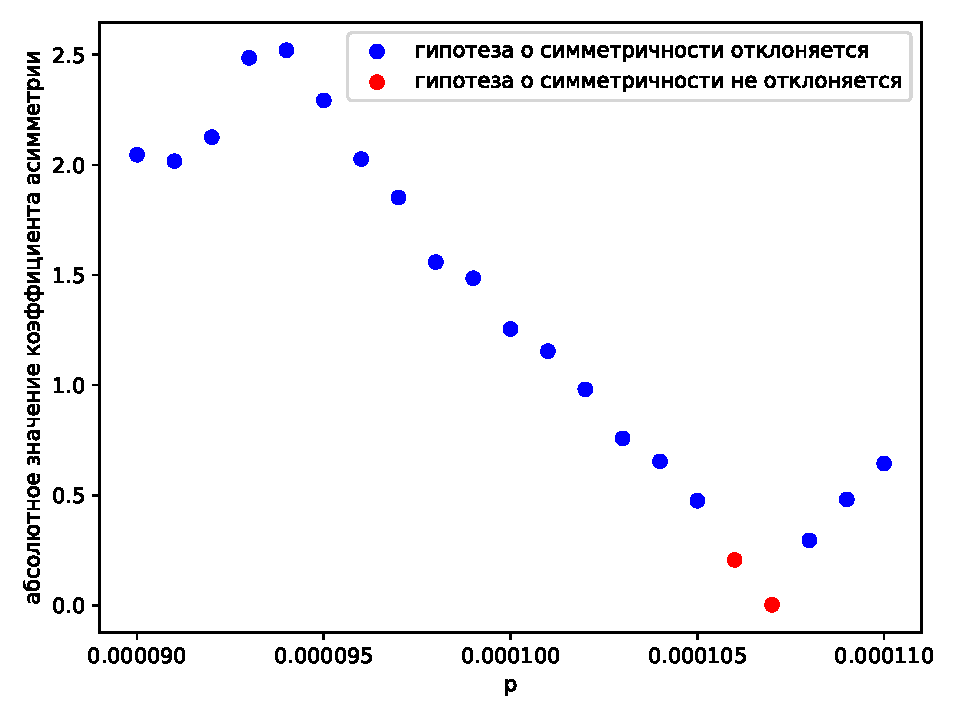
\includegraphics{../../plots/skew_350.pdf} 
     \caption{График изменения абсолютного значения коэффициента асимметрии}
     \label{skew}
\end{figure} 
На рисунке \ref{skew} приведена визуализация вышеописанного 
метода для проверки симметричности распределения размера
наибольшей компоненты связности для модели 
$G(n,p), n =10000, p \in [\frac{1-\epsilon}{n};\frac{1+\epsilon}{n}], \epsilon=0.1$. Как можно заметить 
коэффициент асимметрии значительно отличается от нуля, а 
использование теста только подтверждает отсутствие симметричности.
\subsection{Исследование путей в графах}
Задача поиска самого длинного пути в графе является 
NP-полной, из-за чего оцениваться будет не самый длинный путь, 
а самый длинный найденный путь с помощью поиска в глубину.
Вершины графа, которые находятся в стеке во время 
выполнения поиска в глубину, образуют путь.
\begin{figure}[H] 
    \centering
    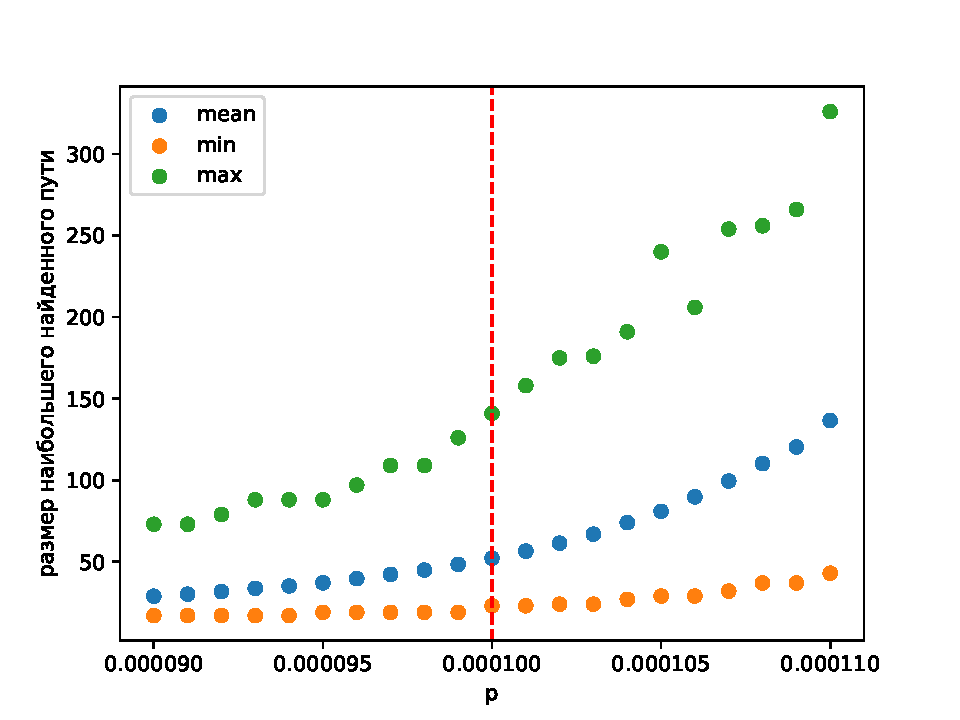
\includegraphics{../../plots/max_path_plot.pdf} 
    \caption{Изменение длины наибольшего найденного пути}
    \label{path_1}
\end{figure} 
\begin{figure}[H] 
\centering
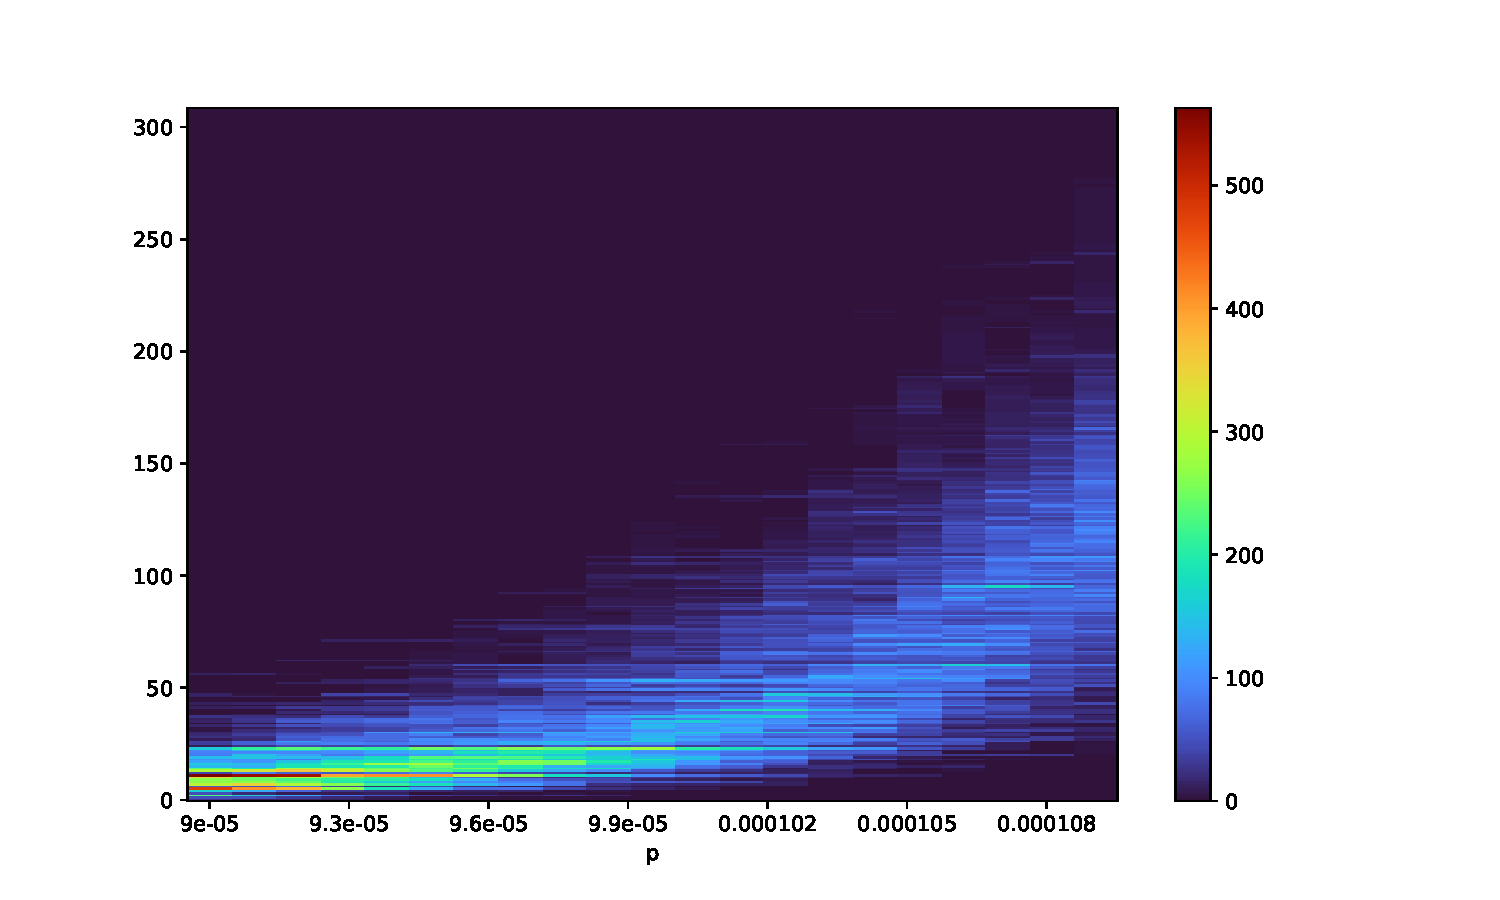
\includegraphics[scale=0.6]{../../plots/hm2.pdf}
\caption{Тепловая карта изменения наибольшего найденного пути}
\label{hm_2}
\end{figure} 
На рисунках \ref{path_1},\ref{hm_2} приведена 
визуализация изменения наибольшего найденного пути 
с помощью поиска в глубину. Графы строились при 
$n = 10000$, $\epsilon =0.1$, $p \in [\frac{1-\epsilon}{n};\frac{1+\epsilon}{n}]$.
На рисунке \ref{path_1} виден характер изменений наибольшего 
найденного пути. Тепловая карта, приведенная на рисунке \ref{hm_2}, описывает более точно характер изменений. Было проведено 350 экспериментов 
при $n = 10000$, $\epsilon \in \{0.1,0.01,0.5\}$. Теорема
об оценке длины найденного пути в графе выполнялась всегда.
\subsection{Проверка длины наибольшего найденного пути на симметричность}
Применим метод проверки выборки на симметричность, описанный в 
разделе \ref{test}. Использовались данные о вычислении 
длины наибольшего найденного пути с помощью поиска в глубину при
$n=10000$,  $\epsilon = 0.1$ , $p \in [\frac{1-\epsilon}{n};\frac{1+\epsilon}{n}]$.
\begin{figure}[H] 
\centering 
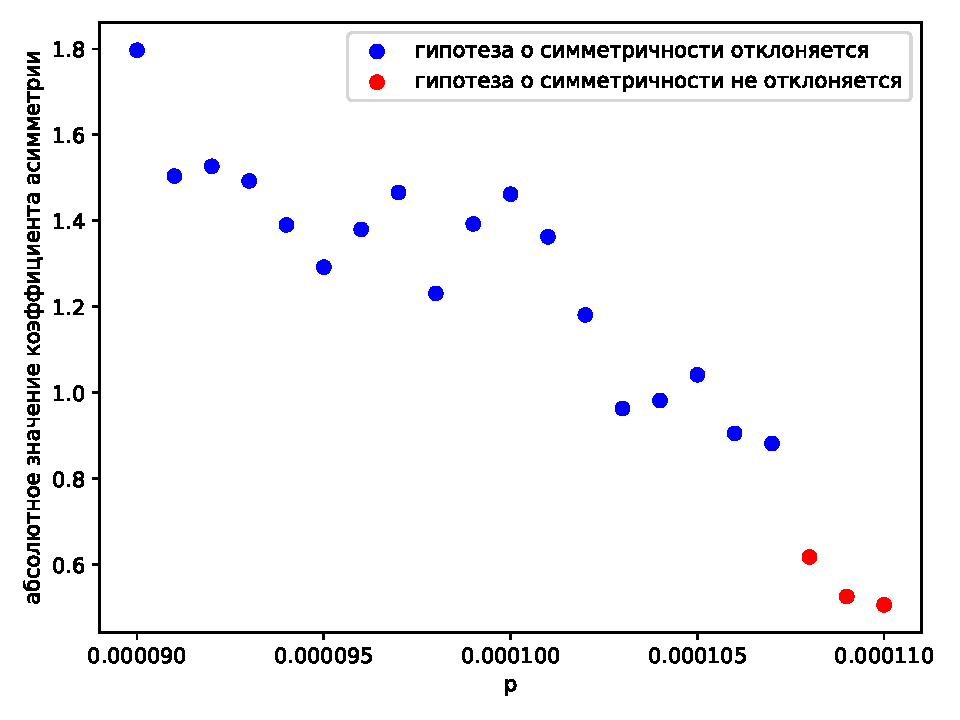
\includegraphics{../../plots/skew_path.pdf}
\caption{Изменение абсолютного значения коэффициента асимметрии}
\label{skew_path}
\end{figure} 
Из графика, представленного на рисунке \ref{skew_path} 
можно заметить, что симметричность в распределении
длин найденных путей не наблюдается.
\subsection{Исследование связности графов}
Были проведены 110 экспериментов, $n=10000$, $p \in [0.1 \frac{\ln{n}}{n} ; 1.2\frac{\ln{n}}{n}]$. Для каждого 
графа вычислялось количество компонент связности. Для 
каждого значения $p$ была вычислена доля связных графов, среди 
всех экспериментов.
\begin{figure}[H] 
    \centering
    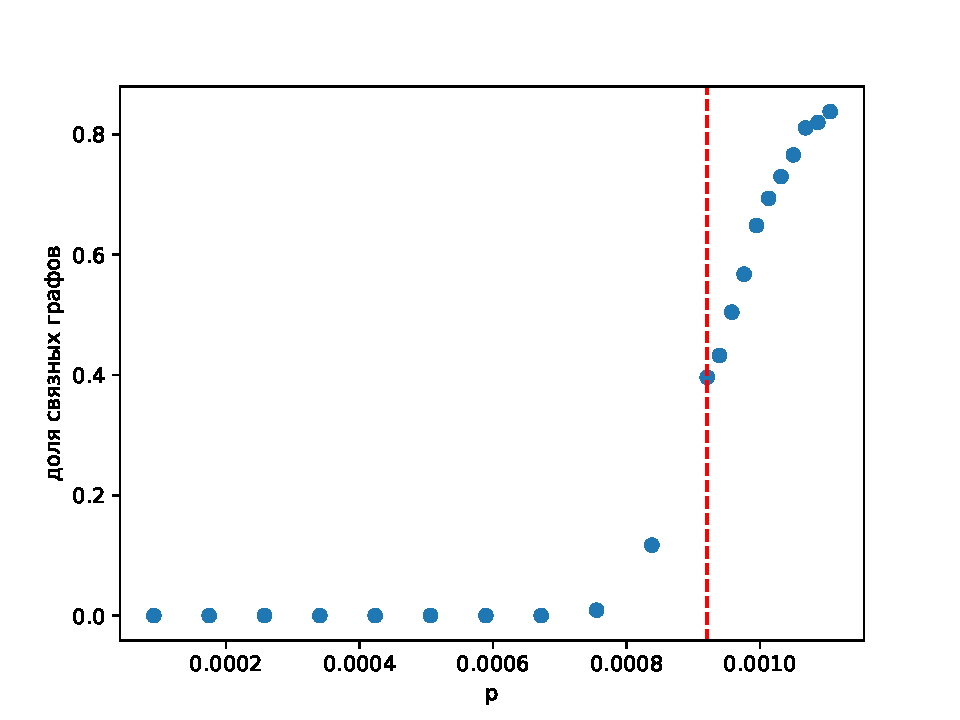
\includegraphics{../../plots/connected.pdf} 
    \caption{Изменение доли связных графов при $p \in [0.1 \frac{\ln{n}}{n};1.2 \frac{\ln{n}}{n}]$}
    \label{con}
\end{figure}  
На рисунке \ref{con} можно заметить фазовый переход 
$p = \frac{\ln{n}}{n}$. Структура построенных графов меняется 
при достижении этого значения.
\subsection{Исследование структуры графов}
Структура графа была исследована путем расчета доли 
деревьев среди всех компонент связности графа. Были проведены 
153 эксперимента, вычислена средняя доля деревьев среди всех экспериментов, $n=10000$, $\epsilon=0.1$.
\begin{figure}[H] 
\centering 
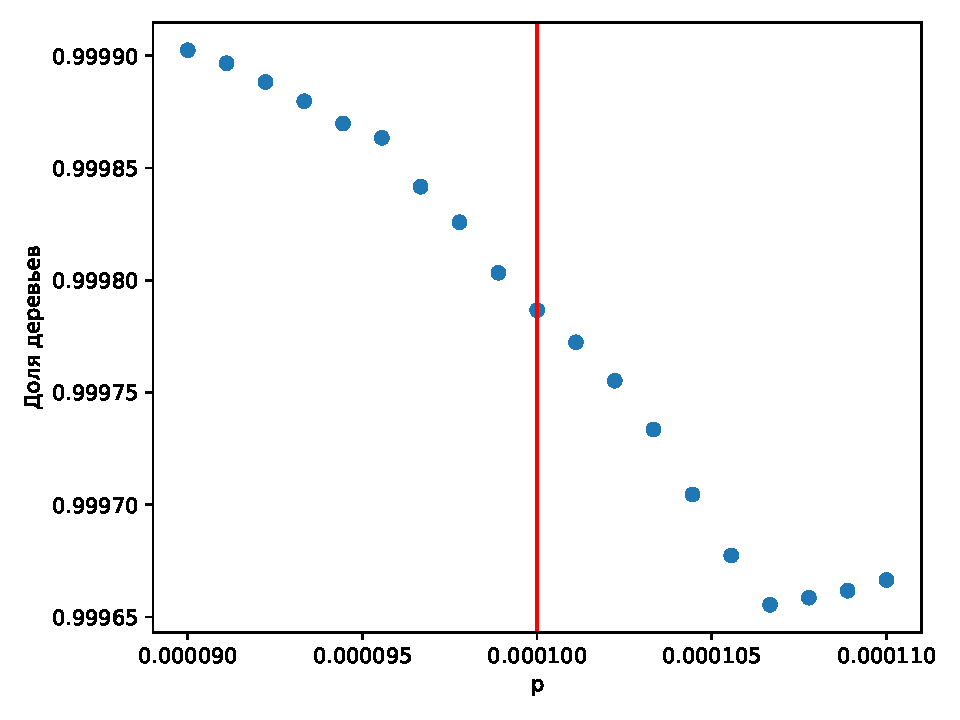
\includegraphics[scale=0.8]{../../plots/tree1.pdf}
\caption{Изменение доли деревьев при $p \in [\frac{1-\epsilon}{n};\frac{1+\epsilon}{n}]$}
\label{tree_1}
\end{figure} 
\begin{figure}[H] 
\centering 
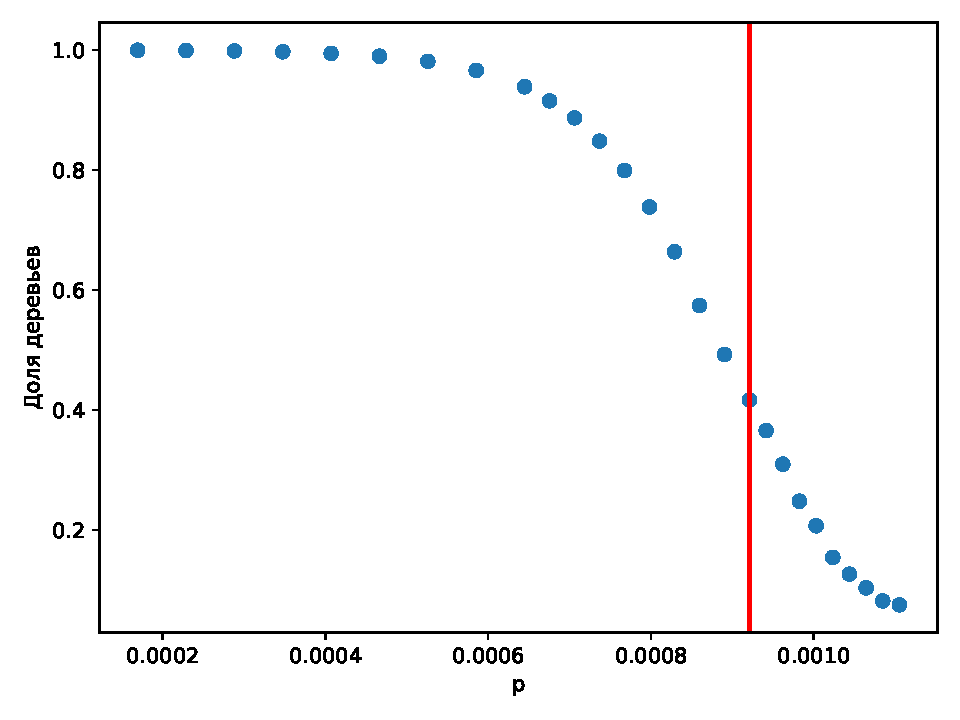
\includegraphics[scale=0.8]{../../plots/tree2.pdf}
\caption{Изменение доли деревьев при $p \in [\frac{1+\epsilon}{n};1.1 \frac{\ln{n}}{n}]$}
\label{tree_2}
\end{figure} 

Из рисунков \ref{tree_1},\ref{tree_2} 
можно заметить, как меняется структура графа. До 
первого фазового перехода $p = \frac{1}{n}$, в графе 
были в основном деревья, после него появилась гигантская компонента связности, которая деревом не является. После второго фазового перехода $p =\frac{\ln{n}}{n}$ в виде деревьев остались немногочисленные изолированные вершины.

\pagebreak
\section*{ЗАКЛЮЧЕНИЕ}
В данной работе было проведено численное исследование модели $G(n,p)$. Были экспериментально подтверждены известные теоретические факты 
о размерах компонент связности, о связности графа, о длине пути.

Теорема о размере компоненты связности при $p = \frac{1+\epsilon}{n}$ выполнялась при $n=10000$, $\epsilon=0.1$ в 
94\% случаях, при $\epsilon = 0.5$ и $\epsilon=0.01$  
выполнялась в 100 \% случаях.

Оба фазовых перехода модели $G(n,p)$ наблюдались в численных экспериментах. После достижения  $p = \frac{1}{n}$ 
в графе появлялась гигантская компонента связности, размер
которой рос достаточно быстро. После достижения 
$p = \frac{\ln{n}}{n}$ доля связных графов среди всех экспериментов достаточно быстро росла.

Тест на симметричность распределения размера наибольших
компонент связности показал отсутствие симметричности 
почти при всех значениях $p$. Такой же результат дал
тест на симметричность распределения длин наибольших найденных путей.

Фазовые переходы также заметны при исследовании структуры графов. 
До первого фазового перехода $p=\frac{1}{n}$ 
графы представляют собой множество деревьев, после 
его достижения начинают появляться подграфы с циклами, 
после второго фазового перехода $p = \frac{\ln{n}}{n}$
из деревьев остаются немногочисленные изолированные вершины.

Таким образом, численное исследование подтвердило теоретические 
свойства модели $G(n,p)$ и продемонстрировало 
существование фазовых переходов. Перспективой дальнейшего исследования является изучение
поведения других моделей случайных графов, таких 
как модель Барабаши-Альберт и модель малого мира Уоттса-Строгаца.
\addcontentsline{toc}{section}{ЗАКЛЮЧЕНИЕ}

\pagebreak
\printbibliography[title=СПИСОК ИСПОЛЬЗОВАННЫХ ИСТОЧНИКОВ]
\addcontentsline{toc}{section}{СПИСОК ИСПОЛЬЗОВАННЫХ ИСТОЧНИКОВ}
\end{document}
